\subsection{Controller Subsystem}
\label{sec:controller_subsystem}
% Why the MCU connects to the internet
In order for our system to be as self and power efficient as
possible from an end-user perspective, it was determined that our product
would require an internet connection to offload remote command-and-control
to an Amazon Web Services EC2 instance (hence referred to as "AWS" and detailed in
\autoref{sec:web_subsystem}). To make the process of operating our product 
as hands-off as possible to end-users, the microcontroller will connect to
the user's home WiFi network for access to AWS. Bluetooth, Zigbee, Thread,
and other short-range 2.4 GHz communication protocols were disfavored over
WiFi, as we predict most users will not have a device dedicated to
connecting our product via such protocols. Long range (LoRa) protocols were
deemed unncessary, as the intended placement of our product is outside, 
near or next to the user's home. We do not expect our product to produce
or receive large amounts of data, so the decreased bandwidth of a
WiFi-enabled product being beyond the outdoor walls of a building
is not a significant drawback to our application. A wired connection
(802.3/Ethernet) was deemed too invasive to the end-user. It is expected
that most, if not all, end-users have a wireless access point and internet
access. Thus, connection via the 802.11/WiFi standard was a natural choice
for our use case.

% How the MCU connects to the internet (local network, LAN -> NAT -> WAN,
% TCP stack)
\paragraph{CC3200 Overview}
The Texas Instruments CC3200-series (hence referred to as the "CC3200", the
"MCU", or the "microcontroller") of microcontrollers are WiFi-enabled
chips with an ARM Cortex-M4 central processor and a WiFi network processor,
along with many useful peripherals and power management modules. This
series of processors is delivered alongside a software development kit
(SDK) provided by Texas Instruments to ease the development of
Internet-of-Things (IoT) applications.

The CC3200's WiFi network processor supports the following
standards/features useful to our development
(see \autoref{cc3220_network_subsystem}):
\begin{itemize}
    \item WiFi standards: 802.11b/g/n
    \item WiFi security: WEP, WPA/WPA2 PSK, WPA2 enterprise, WPA3 personal,
    WPA3 enterprise
    \item WiFi provisioning: SmartConfig, WPS2
    \item IP protocols: IPv4, IPv6
    \item IP addressing: static IP, DHCPv4, DHCPv6
    \item Transport: UDP, TCP, RAW
    \item Host interface: UART, SPI
\end{itemize}
The CC3200's networking subsystem is identical to the CC3220's, and is further detailed in \autoref{cc3220_network_subsystem}.
\begin{figure}[H]
    \caption{CC3220 networking subsystem (\href{https://www.ti.com/lit/ug/swru455m/swru455m.pdf}{CC3200 SimpleLink™ Wi-Fi® and Internet of Things Technical Reference Manual})}
    \label{cc3220_network_subsystem}
    \centering
    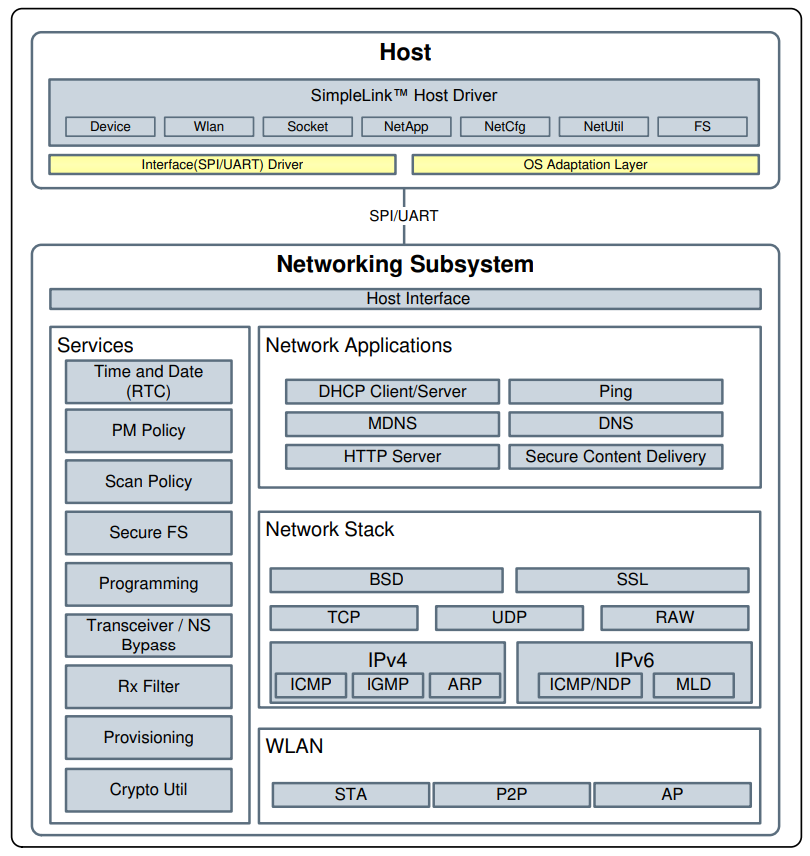
\includegraphics[width=0.75\textwidth]{images/cc3220_network_subsystem.png}
\end{figure}
\paragraph{Connection}
During development of our product, our microcontroller shall connect to a WLAN via a hardcoded password (and username, if needed), or via SmartConfig. The system shall receive an IPv4 address via DHCP, or it shall be able to be statically assigned.

% option a) web interface for user to long in to WLAN
\paragraph{Web Interface Option}
The first option would allow unanimous adaptation of
our product for home users. This option consists of performing first-time
setup through a WiFi Direct connection to the MCU and allowing the user
to login through a web portal to finish setup of their device. The portal
would allow a user to connect to their WLAN of choice, and would
also allow the user to login to the MCU locally to view telemetry and 
settings. The user would also be able to configure the MCU for static
IP addressing or DHCP IP addressing.

% option b) WPS button
\paragraph{WPS Option}
The second option would be to implement a momentary switch which is
programmed to connect to the MCU's WiFi Protected Setup (WPS) feature.
This would still allow the user to connect to their network of
choice---however, the user's wireless access point (WAP) would need to
support WPS. Furthermore, DHCP IP addressing would be forced, and there
would be no web portal for the user to access for viewing telemetry and
settings. This option would greatly ease development, though, and would
let the MCU and web teams focus on developing and refining their
respective subsystems.

% TCP sockets
\paragraph{Communication Method}
The MCU will communicate with AWS through TCP sockets. After connection to
the user's home network, the MCU will check if there is an internet
connection. Once an internet connection has been established, the MCU will
open a socket and connect to the AWS instance via its URL (using the
default DNS nameserver provided to network clients). The software control
flow of TCP sockets as our product will implement them is detailed in
\autoref{tcp_socket_flow}.
\begin{figure}[H]
    \caption{TCP socket control flow (\href{https://www.ti.com/lit/ug/swru368c/swru368c.pdf}{CC3100/CC3200 SimpleLink Wi-Fi Internet-on-a-Chip User's Guide (Rev. C)}, Fig. 5-1)}
    \label{tcp_socket_flow}
    \centering
    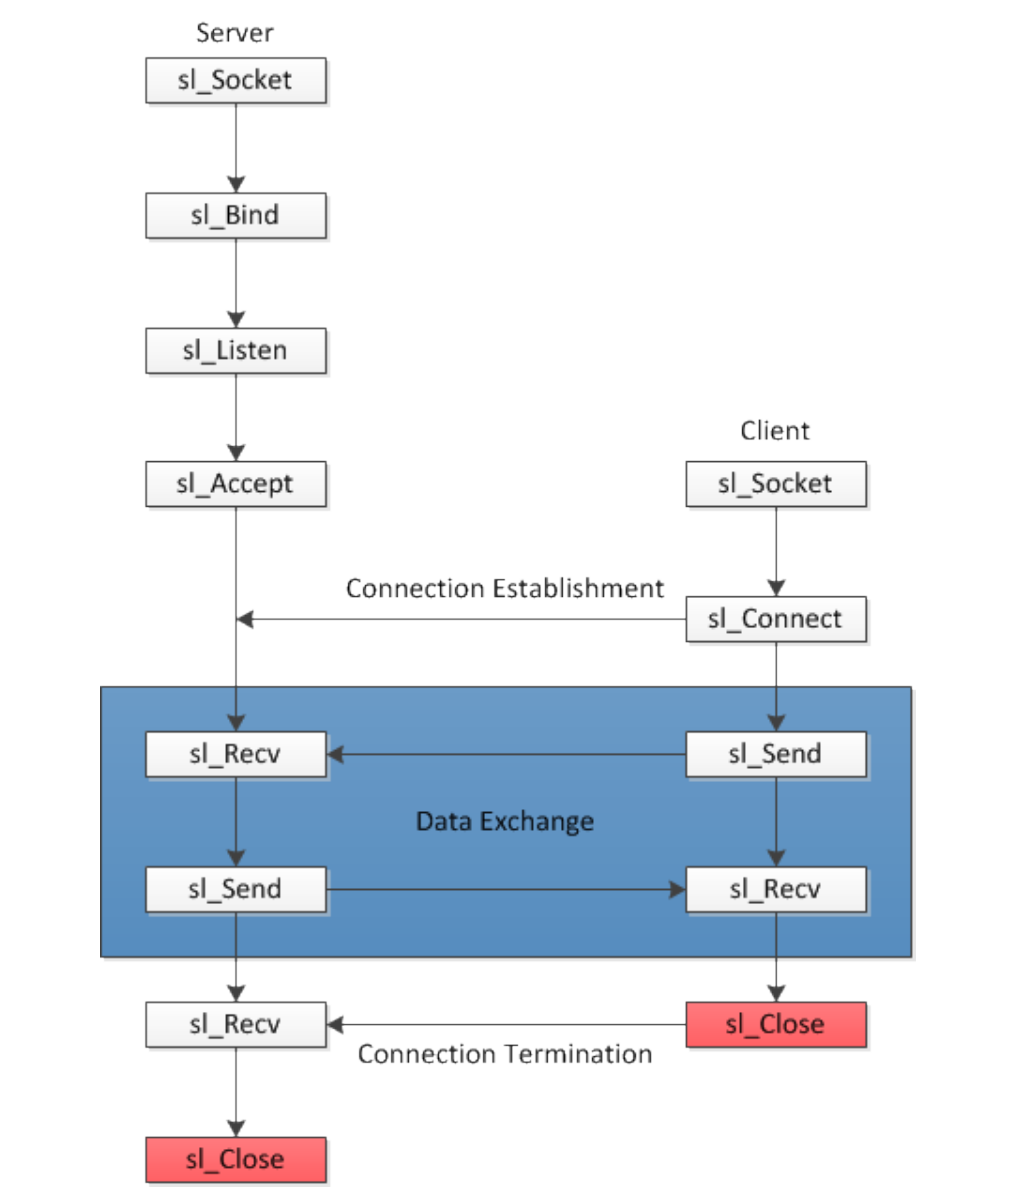
\includegraphics[width=0.8\textwidth]{images/tcp_socket_flow.png}
\end{figure}

% Parameters for connection and how often it tries
\paragraph{Connection Parameters}
Once the MCU has established a connection to the internet and the AWS
instance, it attempts to send current system settings and telemetry, as
well as sensor readings to AWS. The microcontroller does this at least
once every 15 minutes. Sending and receiving may occur more often if
commanded to by AWS. Because TCP is being used to connect AWS and the
microcontroller, any manual retries on a failed send or receive most
likely will be futile. Therefore, any sort of link error handling will
be performed by the link and not the microcontroller program.

% Any over-the-air updates?
\paragraph{Over-the-Air Updates}
At this time, our team does not intend to provide a method for over-the-air
updates (OTA), however, this is a provision that may be developed in the
future.

\paragraph{Startup} Upon startup, the system shall initialize these peripherals in the following order within 30 seconds of startup: watchdog timer, GPIO, ADC, network stack/WiFi module. The system shall then check for interrupts, and execute ISRs if necessary. The system shall then verify its connection to the internet, if set, by attempting to ping \texttt{8.8.8.8} and \texttt{8.8.4.4} 16 at most times over the period of 8 seconds. If 4/16 responses have been received at any point, the system shall attempt to verify network DNS status by pinging \texttt{google.com} 16 at most times over the period of 8 seconds. If 4/16 responses have been received, the system shall continue with startup and clear the no connection flag (if set). If no connection has been established (i.e. the system fails to ping the aforementioned addresses at either step), the system shall set a flag to indicate no connection has been received, and reset. If no connection has been established, and the flag is set, the system shall go into critical power mode and flash the yellow LED for 1 second, 1 time every 2 seconds. The user shall be able to correct the issue via user interface (e.g. SmartConfig or other developed interface). The system shall measure the battery voltage, and set itself to the appropriate state described earlier.

\paragraph{Shutdown} The system shall generate an interrupt to shutdown the system. The shutdown ISR shall run and perform the following actions. The system shall finish any RF transmissions within 5 seconds. The system shall terminate all remaining RF transmissions after the 5 second window has elapsed. The system shall save any network parameters to nonvolatile memory to be used upon startup within 1 second. The system shall safely shutdown any initialized peripherals within 5 seconds. The system shall safely shutdown any sensing components within 5 seconds. The system shall "hand-off" any control it had over the power subsystem to the battery's charge controller within 5 seconds. The system shall go into the shutdown power mode, stopping the processor within 1 second.

\paragraph{Reset} In the event of a reset state, the system shall perform the shutdown ISR, with each section of the ISR performing its necessary tasks within the allotted time mentioned above. The system shall perform its startup ISR, with each section of the ISR performing its necessary tasks within the allotted time mentioned above. There shall be a time period of no longer than 5 seconds between the end of the shutdown ISR and the beginning of the startup ISR.

\paragraph{Networking} The system shall be able to connect to the user's A 2.4 GHz-based wireless network. It may either have no security, or be secured with WPA2 (Personal or Enterprise). The system shall be able to connect if the signal strength of the network is nominal (around -70 dBm). The network shall adhere to the standards of 802.11b, g, or n. The system shall received an IPv4 address assigned by network DHCP, or the user shall be able to statically assign a local IPv4 address. The network shall use NAT, and not expose the product to the WAN. The system shall use DNS provided by the WLAN gateway. The system shall be able to connect to the internet within the timeframe described by the startup sequence. The system shall be ready to establish a connection to AWS within 5 seconds of verifying connection to the internet.

\paragraph{AWS} The system shall first establish a connection to AWS by sending a burst of 5 data packets of the size and containing the variables described in \autoref{toweb_encoding} over a period of 25 seconds. If no connection is established over a period of 15 minutes, the system shall send the same burst of data packets and repeat every 15 minutes until a connection is established.

\paragraph{Receive (Sockets)} The system shall listen for commands from AWS via TCP sockets. If no traffic is received from AWS within a period of 40 minutes, the system shall terminate and attempt to reopen the socket. The system must be able to open and configure a socket within 30 seconds.

\paragraph{Send (Sockets)} The system shall send data to AWS via TCP sockets. If no traffic is successfully sent to AWS within a period of 40 minutes, the system shall terminate and attempt to reopen the socket. The system must be able to open and configure a socket within 30 seconds.

\paragraph{Receive (Command)} While a connection is established with AWS, the system shall continually listen for commands from AWS. The system shall be able to fully receive and decode commands from AWS within 10 seconds of the start of the reception. The system shall be allotted 1 second per command to schedule the received commands.

\paragraph{Send (Data)} While a connection is currently established with AWS, the system shall send a burst of 2 data packets over a period of 10 seconds every 15 minutes. The data packets shall be of the size and contain the variables described in \autoref{toweb_encoding}.

\paragraph{Solar and Battery} The system shall monitor and update the solar array current and voltage output values at least every 10 seconds. The system shall run in active mode between sunrise and sunset, while the battery has 40-100\% calculated charge remaining. The system shall run in low power mode between sunrise and sunset while the battery has 10-40\% calculated charge remaining, and between sunset and sunrise while the battery has 10-100\% calculated charge remaining. The system shall run in critical power mode while the battery has 5-10\% calculated charge remaining. The system shall be in shutdown mode while the battery has 0-5\% calculated charge remaining. The system shall be able to switch power modes within 5 seconds of the interrupt being triggered.
\begin{table}
	\centering
	\begin{tabularx}{\textwidth}
		{
			| >{\raggedright\arraybackslash}X
			| >{\raggedright\arraybackslash}X
			| >{\raggedright\arraybackslash}X
			|
		}
		\caption{MCU power mode behavior}
		\label{table:mcu_battery} \\
		\hline
		\textbf{Time of Day} & \textbf{Calculated Battery Charge (\%)} & \textbf{Power Mode} \\
		\hline
        Day time & 100-40 & Active \\
        \hline
        Night time & 100-40 & Low \\
        \hline
        Any time & 40-10 & Low \\
        \hline
        Any time & 10-5 & Critical \\
        \hline
        Any time & 5-0 & Shutdown \\
        \hline
	\end{tabularx}
\end{table}

\paragraph{Sensing} The system shall monitor and perform analog-to-digital conversion on the spectroscopic sensor values at least every 10 seconds while not in shutdown or critical power mode.

% MCU receives commands, decodes commands
\paragraph{Commands from AWS}
The MCU will receive commands and data from AWS in the following form:
\begin{center}
    \texttt{t x c y}
\end{center}
where \texttt{t} (character) marks the beginning of the command string,
\texttt{x} (unsigned integer) indicates how many seconds to wait before
executing command \texttt{c} (character) with parameter \texttt{y}
(ambiguous). The following characters occupy the spot of \texttt{c}, and
translate to the following commands:
\begin{center}
    \texttt{w y}: water, \texttt{y} is boolean \\
    \texttt{a y}: solar $\theta$, \texttt{y} is double \\
    \texttt{b y}: solar $\phi$, \texttt{y} is double \\
    \texttt{l y}: low power, \texttt{y} is unsigned int for flags \\
    \texttt{s y}: send data, \texttt{y} is unsigned int for flags
\end{center}
For example, if AWS instructs the MCU to turn on the water source in 3
minutes, it would send the command \texttt{t 180 w 1}. If AWS would like
the MCU to change the $\theta$ of the solar panels to 45$\degree$
immediately, it would send \texttt{t 0 a 45.0}. It is important to note
that the values of \texttt{x} and \texttt{y} are not strings (e.g.
45$\degree$ will not be sent as \texttt{"45.0"}), but the actual encoding
of 45$\degree$ as a double-precision float. This is to maintain a
consistent command string size amongst all transmissions.
\begin{figure}[H]
    \caption{Bitwise representation of command}
    \label{command_bitwise}
    \centering
    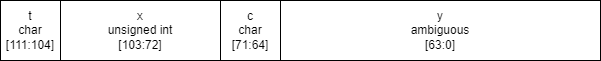
\includegraphics[width=\textwidth]{images/command_encoding.png}
\end{figure}

% Will program in C++. Any libraries, multithreading?
% Singleton Pattern Thread for scheduling tasks
\paragraph{C++ Structure}
It should be expected that all headers from the C++ standard library (as
defined in C++20) will be used, along with the following nonstandard
libraries: Texas Instruments SimpleLink™ CC32xx SDK. Additionally, it is
expected that the MCU program will schedule tasks using a Singleton Pattern
thread to ensure thread safety when accessing variables.

% Classes and class diagram
\paragraph{Classes}
There will be a few classes defined in the MCU's programming, detailed
in \autoref{classes_uml}. Classes will be laid out in the header file
according to the definitions given in the UML diagram.
\begin{figure}[H]
    \caption{UML diagram of the classes used}
    \label{classes_uml}
    \centering
    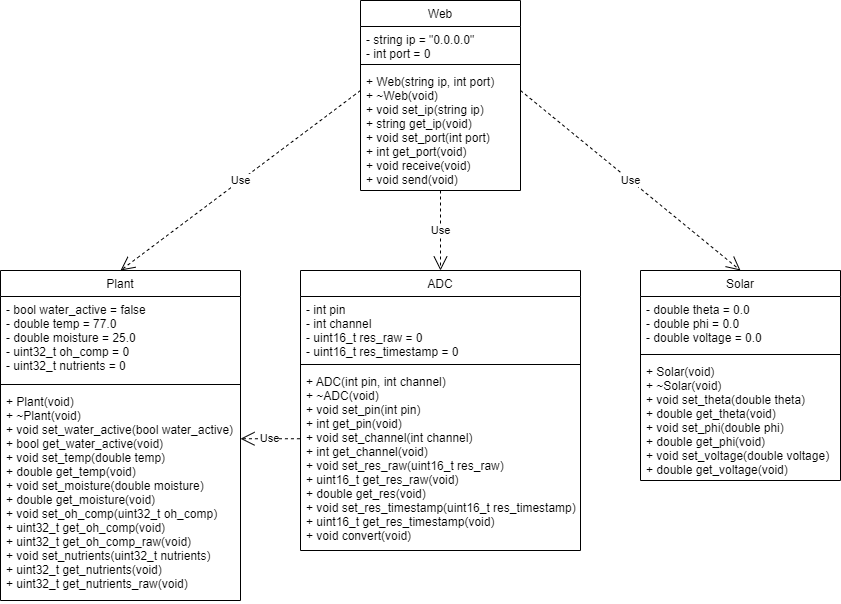
\includegraphics[width=\textwidth]{images/classes_uml.png}
\end{figure}

% Web class
\paragraph{Web Class}
The Web class will have 2 private variables: \texttt{ip} (string) and
\texttt{port} (int). \texttt{ip} signifies the IPv4 address of the AWS instance
to connect to, and \texttt{port} is the port to access AWS through. The default
state of this class is \texttt{ip = "0.0.0.0"} and \texttt{port = 0}. It will
have a public deconstructor and a constructor, requiring the variables string
\texttt{ip} and int \texttt{port} to be passed to the constructor. The class
will have 4 public setters and getters: \texttt{void set\_ip(string ip)},
\texttt{string get\_ip(void)}, \texttt{void set\_port(int port)}, 
\texttt{int get\_port(void)}. The class will have 2 public functions:
\texttt{void receive(void)} and \texttt{void send(void)}.
\texttt{receive()} will be used to receive the next command from AWS, and
will then decode the command and use functions from other classes to execute
the command received from AWS. \texttt{send()} will use functions from
other classes to combine and send the current sensor readings and settings to
AWS. Only 1 object of \texttt{class Web} will be instantiated.

% Plant class
\paragraph{Plant Class}
The Plant class will have 5 private variables: \texttt{water\_active} (bool),
\texttt{temp} (double), \texttt{moisture} (double), \texttt{oh\_comp}
(unsigned 32-bit int), and \texttt{nutrients} (unsigned 32-bit int).
\texttt{water\_active} is the state of the water source feeding the plant,
\texttt{temp} is the current air temperature near/around the plant,
\texttt{moisture} is the moisture percentage of the soil near/around the plant,
\texttt{oh\_comp} is an encoded word of parameters relating to the
spectroscopic analysis of the soil's OH composition, and
\texttt{nutrients} is an encoded word of parameters relating to the
spectroscopic analysis of the soil's nutritional composition. The
default state of this class is \texttt{water\_active = false},
\texttt{temp = 77.0} (room temperature in $\degree$F), \texttt{moisture = 25.0}
(approximate average soil moisture), \texttt{oh\_comp = 0}, and
\texttt{nutrients = 0}. It will have a public deconstructor and a constructor,
requiring no variables to be passed to the constructor. The class will have 12
public setters and getters:
\texttt{void set\_water\_active(bool water\_active)}, 
\texttt{bool get\_water\_active(void)}, 
\texttt{void set\_temp(double temp)}, \texttt{double get\_temp(void)}, 
\texttt{void set\_moisture(double moisture)}, 
\texttt{double get\_moisture(void)}, 
\texttt{void set\_\\
oh\_comp(uint32\_t oh\_comp)}, 
\texttt{uint32\_t get\_oh\_comp(void)},
\texttt{uint32\_t get\_oh\_\\
comp\_raw(void)}, 
\texttt{void set\_nutrients(uint32\_t nutrients)}, 
\texttt{uint32\_t get\_\\
nutrients(void)}, and
\texttt{uint32\_t get\_nutrients\_raw(void)}. The purpose of the normal getters
for \texttt{oh\_comp} and \texttt{nutrients} are to get human-readable formats
for the OH composition of, and nutrients in the soil. The raw getters are to
get the raw values of \texttt{oh\_comp} and \texttt{nutrients}. The setters
accept the raw values of \texttt{oh\_comp} and \texttt{nutrients}. Only 
1 object of \texttt{class Plant} will be instantiated.

% ADC class
\paragraph{ADC Class}
The ADC class will have 4 private variables: \texttt{pin} (int), 
\texttt{channel} (int), \texttt{res\_raw} (unsigned 16-bit int), and
\texttt{res\_timestamp} (unsigned 16-bit int). \texttt{pin} is the physical
pin of the voltage input to the ADC on the CC3200, \texttt{channel} is the
ADC channel corresponding to the selected pin. \texttt{res\_raw} is the raw
result of the ADC for the corresponding channel. \texttt{res\_timestamp} is the
timestamp of the ADC result for the corresponding channel. The default state
of this class is \texttt{res\_raw = 0} and \texttt{res\_timestamp = 0}. It will
have a public deconstructor and a constructor, requiring the variables int
\texttt{pin} and int \texttt{channel} to be passed to the constructor.
The class will have 9 public setters and getters:
\texttt{void set\_pin(int pin)}, \texttt{int get\_pin(void)},
\texttt{void set\_channel(int channel)}, \texttt{int get\_channel(void)},
\texttt{void set\_res\_raw(uint16\_t res\_raw)},
\texttt{uint16\_t get\_res\_raw(void)},
\texttt{double get\_\\
res(void)},
\texttt{void set\_res\_timestamp(uint\_16t res\_timestamp)},
\texttt{uint16\_t get\_\\
res\_timestamp(void)}. The \texttt{get\_res()} getter
converts the raw result of the ADC into a voltage. The class will have 1 public
function: \texttt{void convert(void)}. This function manually triggers
conversion in the ADC module of the CC3200. Multiple objects of
\texttt{class ADC} will be instantiated.

% Solar class
\paragraph{Solar Class}
The Solar class will have 1 private variable: \texttt{voltage} (double). \texttt{voltage} is the voltage of the battery updated at
regular intervals. The default state of this class is \texttt{voltage = 0.0}. It will have a public
deconstructor and a constructor, requiring no variables to be passed to the
constructor. The class will have 2 public setters and getters:
\texttt{void set\_voltage(double voltage)}, and
\texttt{double get\_voltage(void)}. Only 
1 object of \texttt{class Solar} will be instantiated.

% Send to AWS, format and types of commands
% Send straight data from the struct
\paragraph{Data to AWS}
Unlike commands received from AWS, the MCU will simply send data directly
from its classes to AWS. This is done to minimize the overhead of sending
extraneous symbols and preserve power stored in the battery, as receiving
uses far less power than transmitting in the MCU subsystem. Further
optimization can be performed in the future to further reduce overhead
(e.g. reducing \texttt{water\_active} to occupy 1 bit and using the rest of
the symbol to encode other data).
\begin{figure}[H]
    \caption{Bitwise representation of data sent to AWS}
    \label{toweb_encoding}
    \centering
    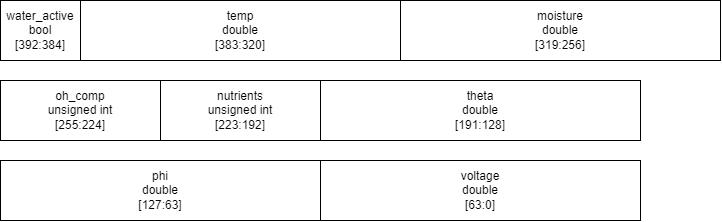
\includegraphics[width=\textwidth]{images/toweb_encoding.png}
\end{figure}

% Global vars
\paragraph{Global Variables}
No global variables plan to be implemented at this time. Macros may be
defined for configuration of the ADC and any other dependent modules.

% Interrupts and ISRs
\paragraph{Interrupts and ISRs}
If the charge controller indicates that the battery has fallen below a
certain voltage (named "low voltage"), the MCU will raise an interrupt and
execute \texttt{isr\_low\_power()}. This ISR performs housekeeping before
putting the MCU into a low power state, limiting use of its functions and consuming less current.

If the charge controller indicates that the battery has fallen below a
certain voltage (named "critical voltage"), the MCU will raise an interrupt
and execute \texttt{isr\_critical\_power()}. This ISR performs further 
housekeeping before putting the MCU into an extreme low power state,
limiting all but the features necessary to maintain a connection with AWS and consuming a minimal amount of current.

If the MCU, AWS, or any other devices transmit indication of a dangerous
state or if the MCU, AWS, or any other devices transmit indication of a
shut down, the MCU will raise an interrupt and execute
\texttt{isr\_shut\_down()}. This ISR immediately shuts down all able
subsystems, and puts all other subsystems in a fail safe state. This ISR
fails safe the entire system.

If the MCU receives indication of a start up (via a momentary switch), the
MCU will raise an interrupt and execute \texttt{isr\_start\_up()}. This ISR
starts up all relevant subsystems and begins the MCU's programming. All
classes will be initialized to default values. This ISR starts up the
entire system.

If the MCU determines it must reset the system to a default state, the
MCU will raise an interrupt and execute \texttt{isr\_default\_state()}.
This ISR returns all relevant subsystems to their default state,
as if the MCU had just executed \texttt{isr\_start\_up()}. All classes will
be initialized to default values. This ISR resets the entire system.

If the watchdog timer needs to be reset to 0 in the course of normal operation, the triggered interrupt shall execute \texttt{isr\_wdt()} to reset the WDT.

% File organization (main, header files, other source files, etc.)
\paragraph{File Organization}
Classes, macros, functions, and variables will be defined/prototyped to the
extent required in a header file to be named \texttt{garden.h}. These
classes, functions, and variables will be further defined in a seperate
source file named \texttt{garden.cpp} as needed. The \texttt{main()}
function and the remaining classes, macros, functions, and variables,
required will be located in \texttt{main.cpp}.

% How the MCU gets data from sensors (ADC)
\paragraph{Analog-to-digital Conversion}
The CC3200 contains a 12-bit general purpose analog-to-digital converter
(ADC) with 4 externally-accessible channels and a sampling periodicity of
16 $\upmu$s per channel (62.5 ksps per channel). The architecture of the
CC3200's ADC is shown in \autoref{cc3200_adc_arch}.
\begin{figure}[H]
    \caption{CC3200 ADC module architecture (\href{https://www.ti.com/lit/an/swra679/swra679.pdf}{SimpleLink™ Wi-Fi® CC32xx ADC}, Fig. 1-2)}
    \label{cc3200_adc_arch}
    \centering
    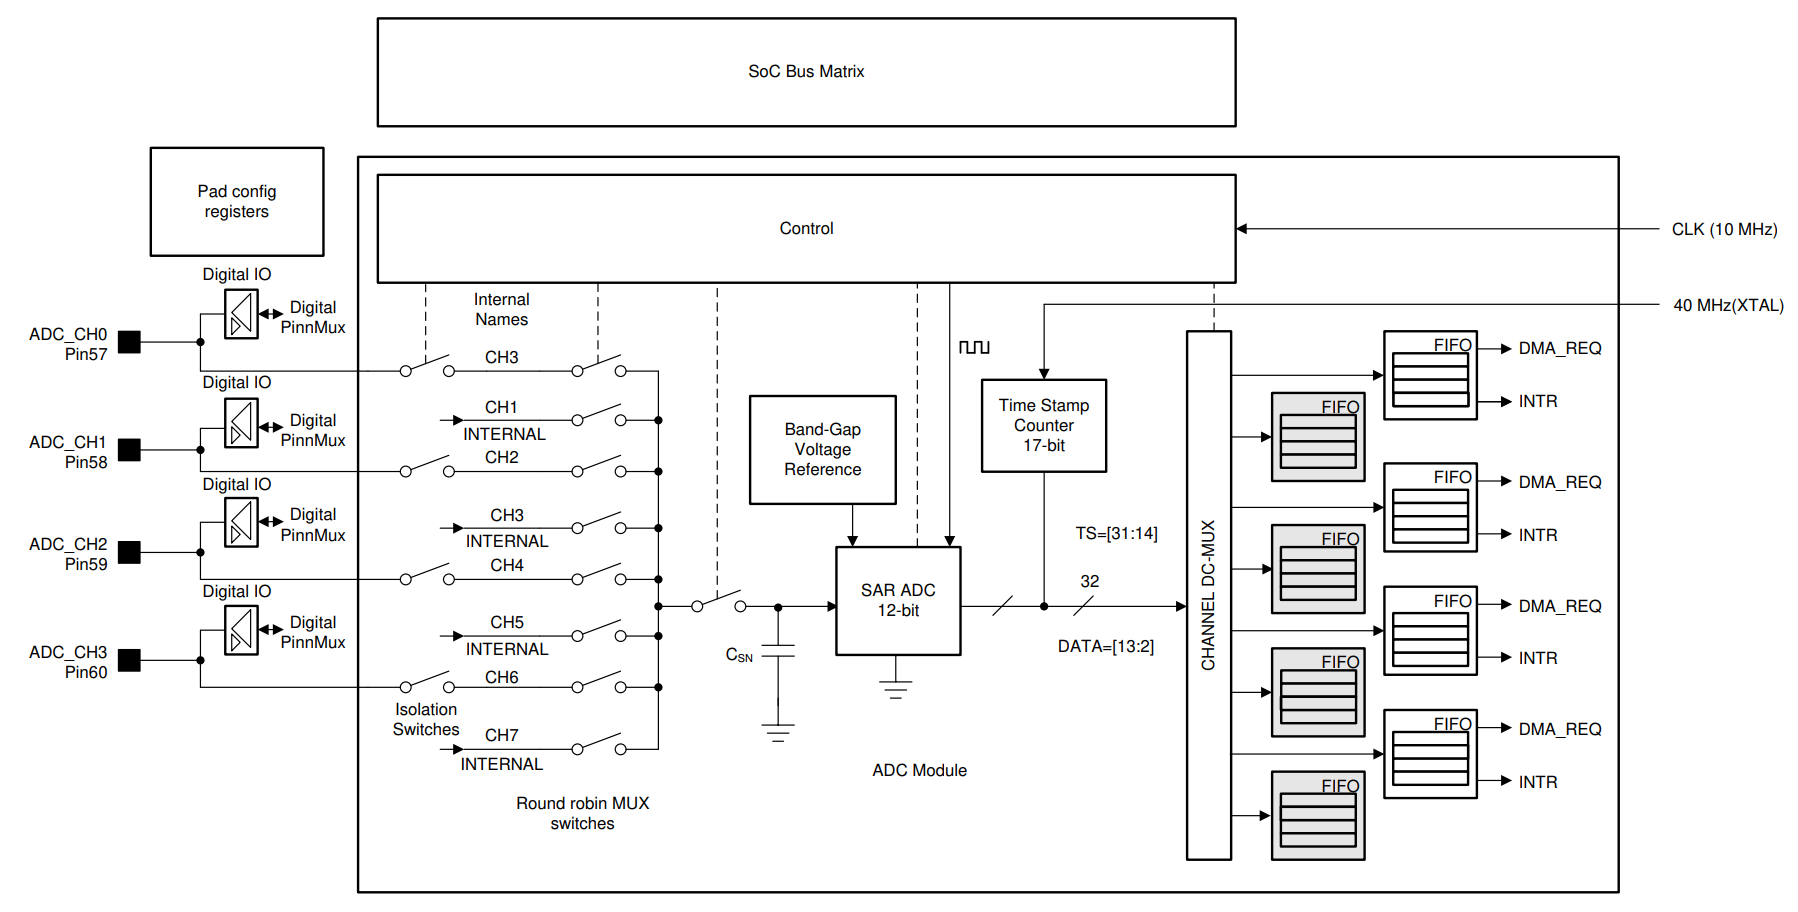
\includegraphics[width=\textwidth]{images/cc3200_adc_arch.png}
\end{figure}

% How the MCU gets data from sensors (ADC, cont.)
It is expected that the spectrometer circuit will provide a current
between 20 $\upmu$V and 80 mV. The 12-bit ADC provides for an input range of
between 0 and 1.8 V. Therefore, the resolution of the ADC is calculated
below:
\begin{equation}
    \label{eq:adc_res}
    \frac{(1.8 - 0)\,\mathrm{V}}{2^{12}\,\mathrm{steps}} =
    0.4395\,\mathrm{mV}/\mathrm{step}
\end{equation}
Thus, given our ADC resolution and the expected range of our spectrometer,
the number of discrete steps of range is given below:
\begin{equation}
    \label{eq:adc_steps}
    \frac{(80 - 0.02)\,\mathrm{mV}}{0.4395\,\mathrm{mV}/\mathrm{step}} =
    \lfloor181.98\rfloor = 181
\end{equation}
These steps will be used to measure OH composition and nutrients in the
soil, and functions from the class \texttt{ADC} will be used to perform
analog-to-digital conversion to update values in the class \texttt{Plant}.

In the future, a more precise ADC module could be explored to give the
CC3200 more resolution when performing spectroscopy.

% How MCU sends data to servos
\paragraph{Communication with Servos}
The MCU will directly control GPIO and bit-bang values to the servo motors
controlling the orientation of the solar panels when using functions from
the class \texttt{Solar}. This method of control may be refined further in
the future.

% What sort of telemetry we'll have
\paragraph{Telemetry}
No data that would be exclusively considered telemetry will be transmitted 
between AWS and the MCU (e.g. processor temperature). Instead, all
"telemetry" values will be handled with interrupts and ISRs/functions
on-chip, while current settings and sensor readings will be transmitted
back to AWS.

% What kind of development model?
\paragraph{Development Model}
An Agile development model will be used. Code reviews will be performed on
an as-needed basis by a convening of members of the MCU subsystem and the
web subsystem teams.
\begin{figure}[H]
    \caption{UML diagram of the subsystem's development methodology}
    \label{mcu_agile_uml}
    \centering
    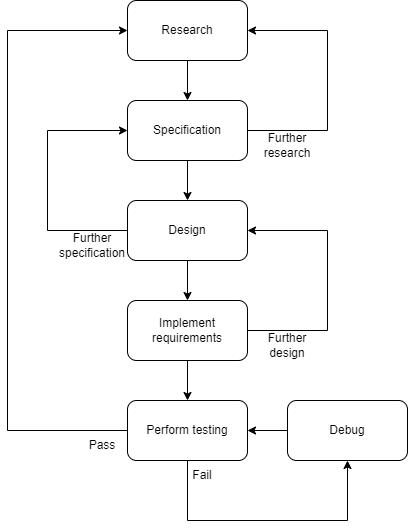
\includegraphics[width=0.65\textwidth]{images/mcu_agile_uml.png}
\end{figure}

% IDE and Git
\paragraph{IDE and Git}
Texas Instruments Code Composer Studio v12 will be used to program,
compile (via TI ARM compiler v20), and debug the C++-based project. GitHub
will be used as a repository for the project, using Git for version
control.

% Power
\paragraph{Power}
The MCU will be connected to power from the power subsystem detailed in 
\autoref{sec:power_subsystem}. It is expected to receive 3.3 V, and this will
be fed to the integrated DC/DC converter on the CC3200. The converter is able
to convert voltages from 2.3 to 3.6 V.

% Pinout 
\paragraph{Pinout Diagram}
The CC3200 will connected to the following components as described by the
pinout diagram shown in \autoref{CC3200_pinout}.
\begin{figure}[H]
    \caption{CC3200 pinout diagram (red labels indicate pins will be connected to other components in a way that differs from the reference design)}
    \label{CC3200_pinout}
    \centering
    \includegraphics[width=\textwidth]{images/CC3200_pinout.png}
\end{figure}

% LEDs
\paragraph{LEDs} The system shall be able to make use of its onboard LEDs for notifying the user or developers of system states. When the system is in active mode, the green LED shall be solidly illuminated. When the system is in low power mode, the green LED shall flash 1 time for a period of 0.5 seconds, every 2 seconds. When the system is in critical power mode, the red LED shall flash 2 times for a period of 0.5 seconds per flash, seperated by 1 second between each flash, every 30 seconds. When the system is in shutdown mode, no LEDs shall be active. When the system is starting up, the green and red LED shall be solidly illuminated until the startup sequence is completed and the system transitions into a different power mode. The yellow LED shall solidly illuminate while receiving data through the RF antenna for
the duration of the reception. The yellow LED shall blink 1 time every 0.2 seconds for a period of 0.1 second while transmitting data through the RF antenna for the duration of the transmission.

\begin{table}
	\centering
	\begin{tabularx}{\textwidth}
		{
			| >{\raggedright\arraybackslash}X
			| >{\raggedright\arraybackslash}X
			| >{\raggedright\arraybackslash}X
			| >{\raggedright\arraybackslash}X
			|
		}
		\caption{MCU LED operation}
		\label{table:mcu_leds} \\
		\hline
		\textbf{Power Mode} & \textbf{Red LED} & \textbf{Yellow LED} & \textbf{Green LED} \\
		\hline
        \textbf{Active} & Not active & RX: Solidly illuminated, TX: 1 flash of 0.1 s, every 0.2 s & Solidly illuminated \\
        \hline
        \textbf{Low} & Not active & RX: Solidly illuminated, TX: 1 flash of 0.1 s, every 0.2 s & 1 flash of 0.5 s, every 2 s \\
        \hline
        \textbf{Critical} & 2 flash of 0.5 s, 1 s seperation, every 30 s & No connection: 1 flash of 1 s, every 2 s & Not active \\
        \hline
        \textbf{Shutdown} & Not active & Not active & Not active \\
        \hline
        \textbf{Startup} & Solidly illuminated & Not active & Solidly illuminated \\
        \hline
	\end{tabularx}
\end{table}

% Watchdog
\paragraph{Watchdog Timer} The CC3200 has an onboard watchdog timer used to detect and recover from freezes, crashes, or lockups. When the watchdog timer reaches zero, the watchdog module shall trigger an interrupt. The ISR triggered by the interrupt shall reset the watchdog timer. In the case the ISR is not able to be triggered by the interrupt (e.g. system freeze), the watchdog module shall reset the system. After the system is reset by the watchdog module, the system shall start up normally.

% PCB
\paragraph{Printed Circuit Board} Our controller subsystem will be developed and implemented on a Texas Instruments \href{https://www.ti.com/tool/CC3200SF-LAUNCHXL}{CC3200SF-LAUNCHXL} LaunchPad development board with a plug-in daughterboard hat containing sensing and other components. In an ideal scenario, our team would like to develop a custom PCB for our controller subsystem---however, decreased supply and increased lead times, as well as the extra time needed to develop, test, and implement a PCB forced our hand to use the development board in the final product.

If Texas Instruments' global integrated circuit supply increases and MCUs become more available, and our team is on-time with project goals and objectives, we would like to explore design of a PCB for the controller subsystem. Because the product is using the reference design currently, our team does not yet have a custom schematic for the controller subsystem. Thus, our product's schematic  may be found in \autoref{mcu_pcb_schematic}.
\begin{figure}[H]
    \caption{MCU subsystem schematic}
    \label{mcu_pcb_schematic}
    \centering
    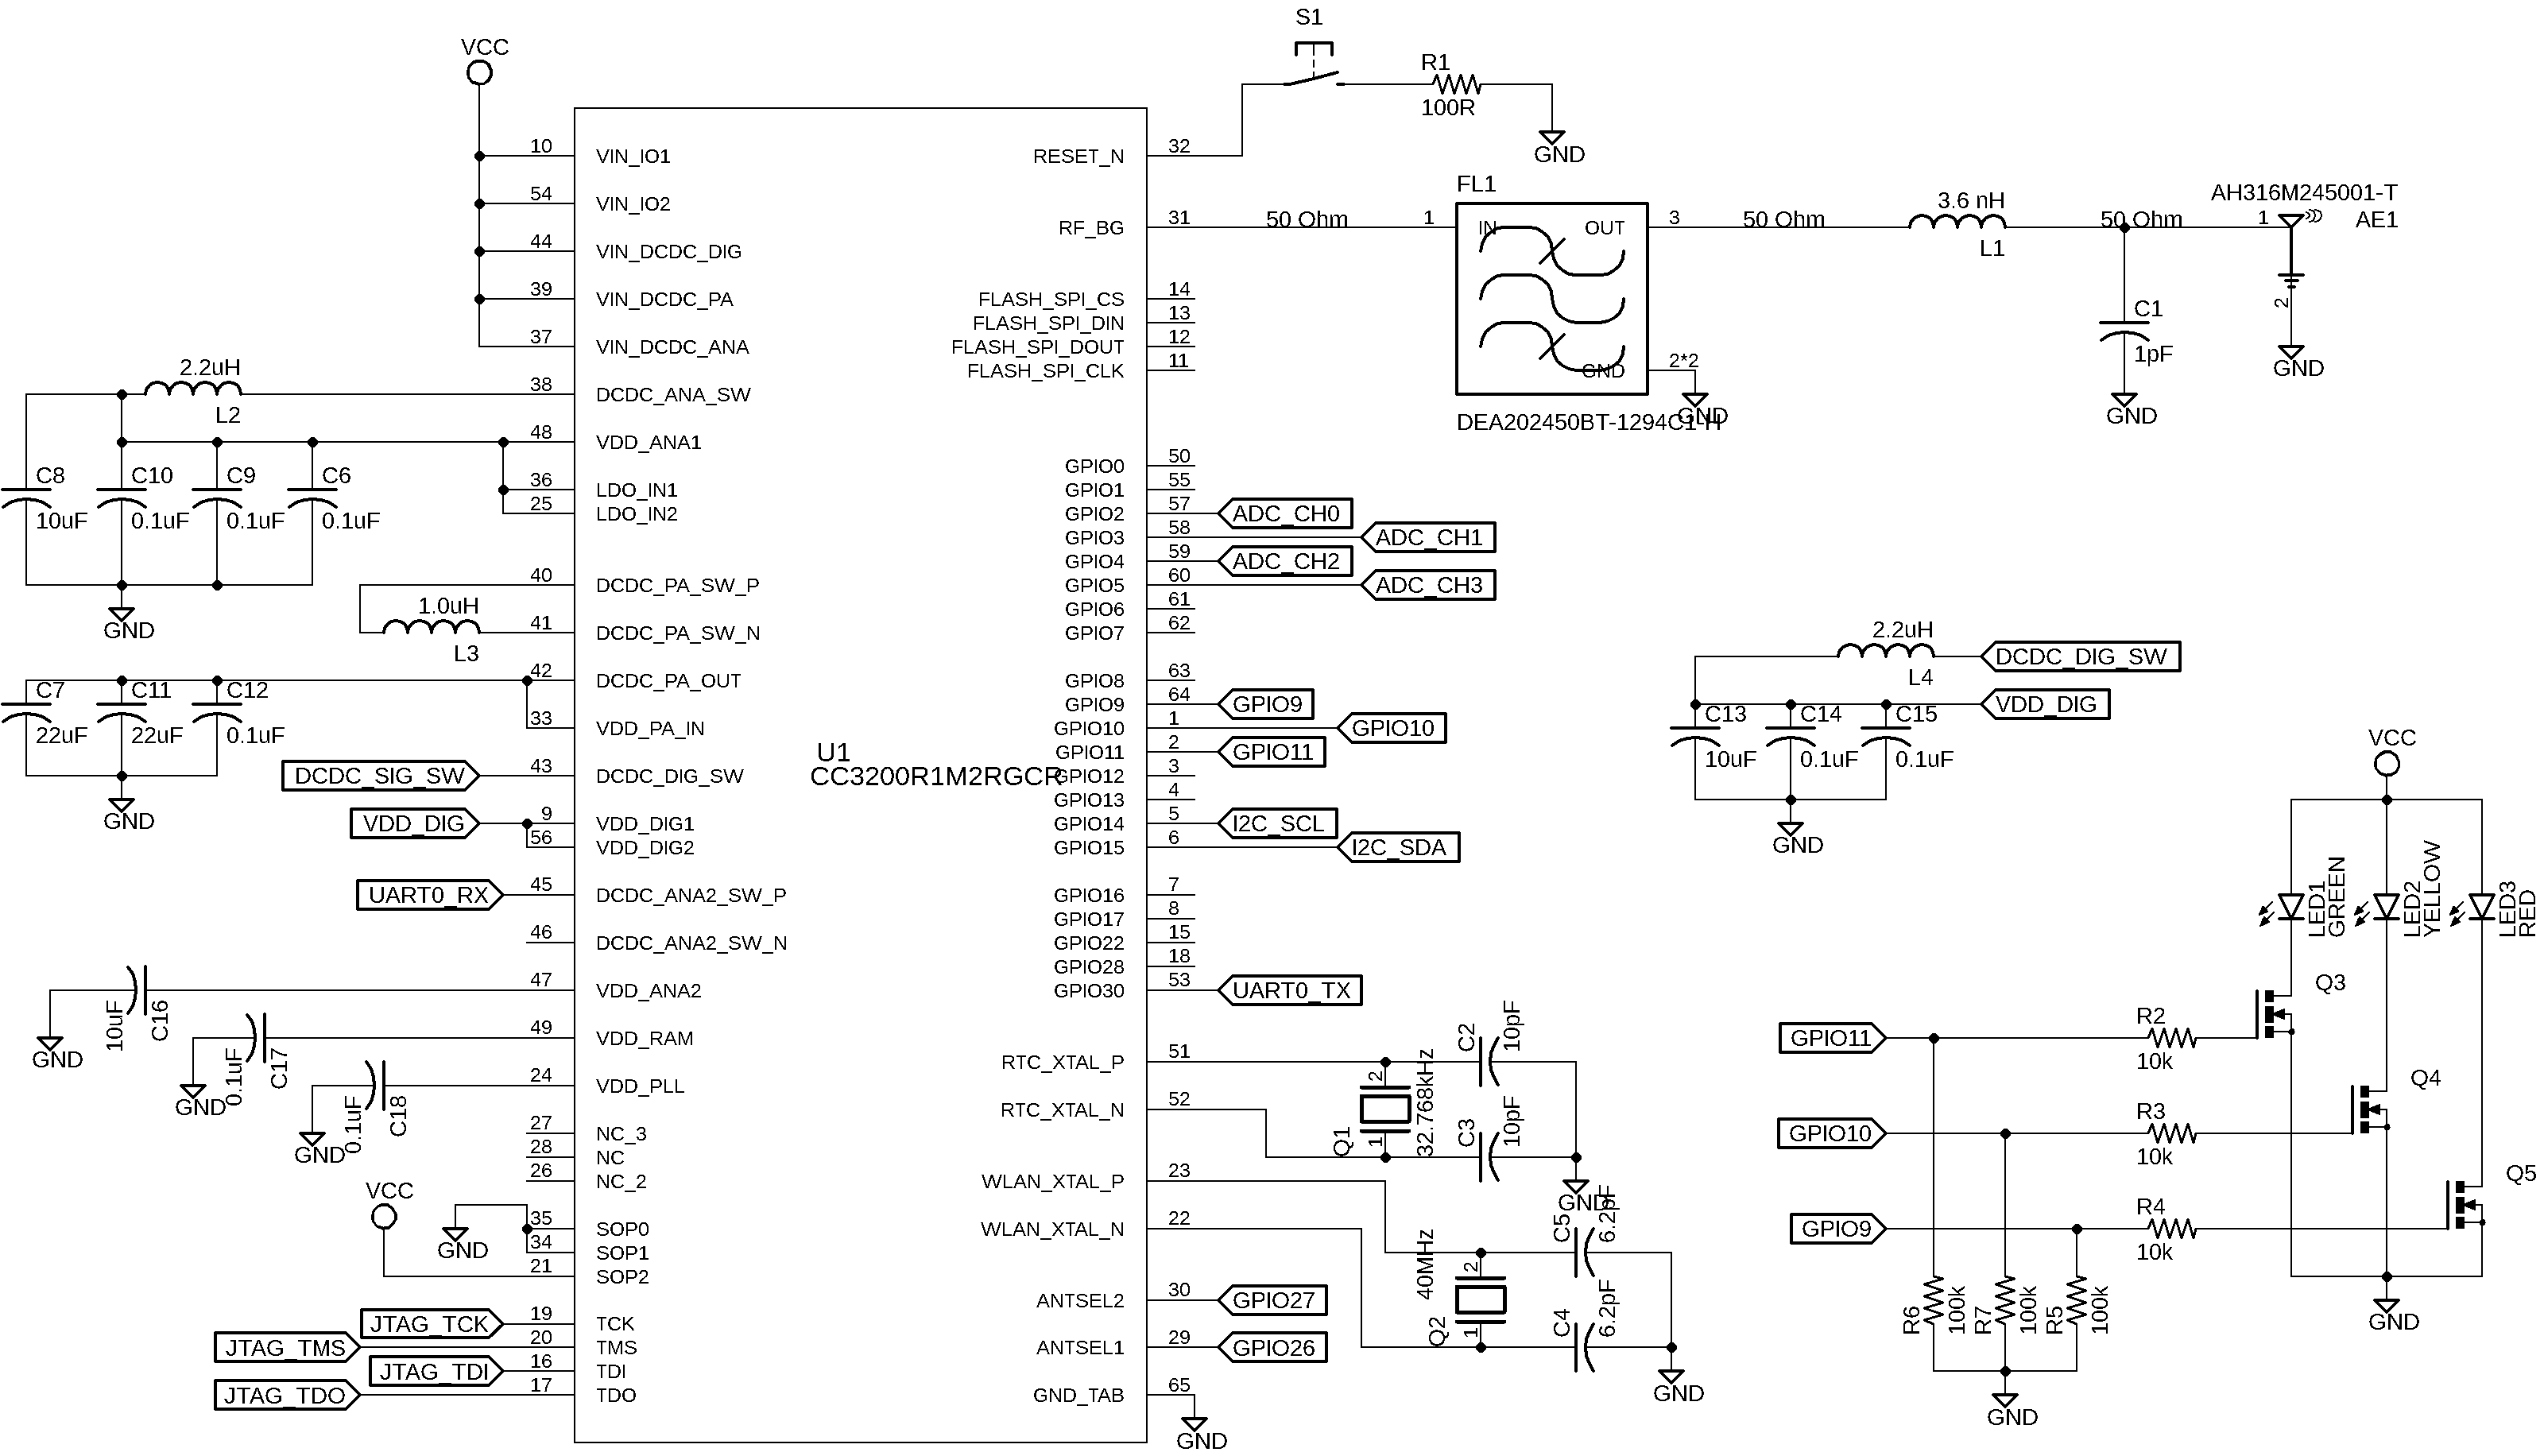
\includegraphics[width=\textwidth]{images/mcu_pcb_schematic.png}
\end{figure}